\usetikzlibrary{arrows.meta,calc}
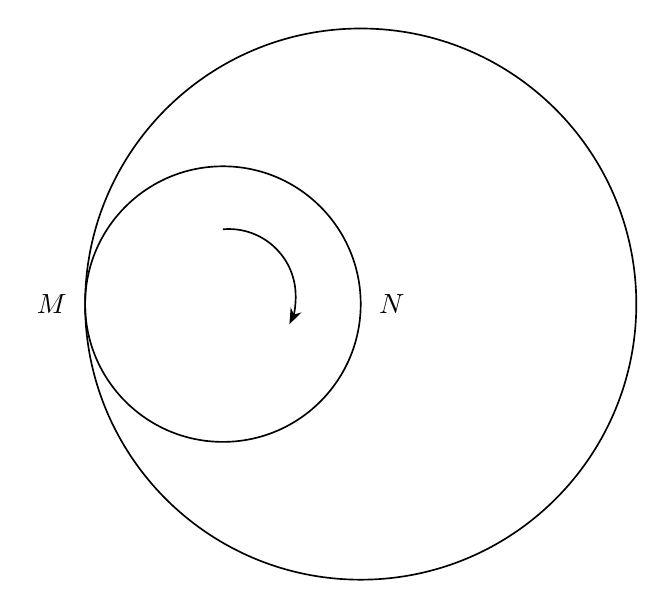
\begin{tikzpicture}[x=1cm,y=1cm,line width=.6pt,font=\normalsize,>=Stealth]
\coordinate (O_big) at (0,0);
\coordinate (O_small) at (-1.75,0);
\coordinate (M) at (-3.5,0);
\coordinate (N) at (0,0);
\draw (O_big) circle[radius=3.5cm];
\draw (O_small) circle[radius=1.75cm];
\draw[->] (-1.75,0.95) arc[start angle=95,end angle=-25,radius=0.85cm];
\node[left,xshift=-3pt] at (M) {$M$};
\node[right,xshift=3pt] at (N) {$N$};
\end{tikzpicture}
